\documentclass[crop,tikz]{standalone}
\usepackage[usenames]{color} %used for font color
\usepackage{amssymb} %maths
\usepackage{amsmath} %maths
\usepackage[utf8]{inputenc} %useful to type directly diacritic characters
\usepackage{tikz}
\usetikzlibrary{calc,arrows,patterns,intersections}
\usetikzlibrary{shapes.multipart}
\usepackage{pgfplots}
\usepgfplotslibrary{fillbetween}
\pgfmathdeclarefunction{gauss}{2}{%
  \pgfmathparse{1/(#2*sqrt(2*pi))*exp(-((x-#1)^2)/(2*#2^2))}%
}
\begin{document}

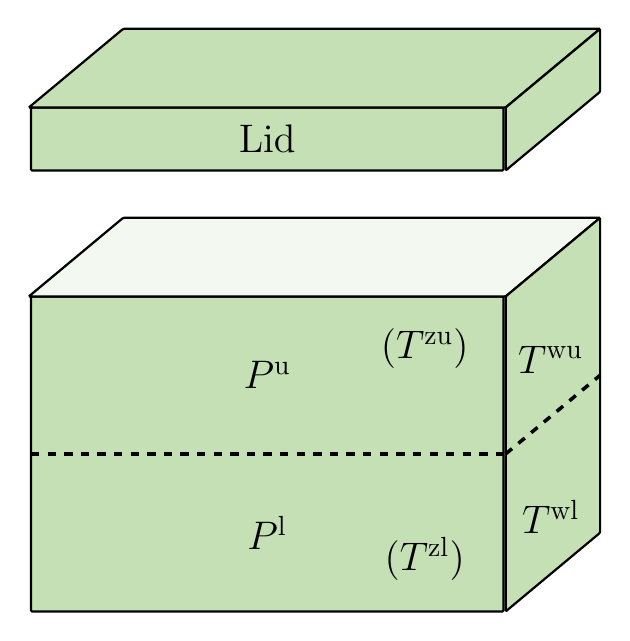
\begin{tikzpicture}
  \definecolor{CUBE}{RGB}{197,224,180};
  % Settings
  \coordinate (CenterPoint) at (0,0);
  \def\width{6.0cm};
  \def\height{4.0cm};
  \def\textborder{1.0cm};
  \def\xslant{1.2cm};
  \def\yslant{1.0cm};
  \def\rounding{0.4pt};
  % Drawing
  \node[thick, draw,
    minimum height  = \height,
    minimum width   = \width,
    text width      = {\width-1*\textborder},
    align           = center,
    fill            = CUBE,
    rounded corners = \rounding]
  at (CenterPoint) {}; % TEXT HERE?

  \draw[name path=HorizontalDashedLine, dashed, line width=0.45mm, black]%
  ($(CenterPoint) + (-\width/2., 0)$) -- ($(CenterPoint) + (\width/2., 0)$);

  % "3D" top
  \draw [rounded corners = \rounding, thick, fill=CUBE!20] %
  ($(CenterPoint) + (-\width/2. - 2*\rounding, \height/2.)$) -- %
  ($(CenterPoint) + (-\width/2. + \xslant - 2*\rounding, \height/2. + \yslant)$) -- %
  ($(CenterPoint) + (\width/2. + \xslant + 2*\rounding, \height/2. + \yslant)$) -- %
  ($(CenterPoint) + (\width/2. + 2*\rounding, \height/2.)$) -- %
  cycle;
  % "3D" side
  \draw [rounded corners = \rounding, thick, fill=CUBE] %
  ($(CenterPoint) + (\width/2. + \xslant + 2*\rounding, \height/2. + \yslant)$) -- %
  ($(CenterPoint) + (\width/2. + 2*\rounding, \height/2.)$) -- %
  ($(CenterPoint) + (\width/2. + 2*\rounding, -\height/2.)$) -- %
  ($(CenterPoint) + (\width/2. + \xslant + 2*\rounding, -\height/2. + \yslant)$) -- %
  cycle;

  \coordinate (CenterPointLid) at (0,4);
  \node[thick, draw,
    minimum height  = \height*0.2,
    minimum width   = \width,
    text width      = {\width-1*\textborder},
    align           = center,
    fill            = CUBE,
    rounded corners = \rounding]
  at (CenterPointLid){\Large Lid};

  \draw [rounded corners = \rounding, thick, fill=CUBE] %
  ($(CenterPointLid) + (-\width/2. - 2*\rounding, 0.2*\height/2.)$) -- %
  ($(CenterPointLid) + (-\width/2. + \xslant - 2*\rounding, 0.2*\height/2. + \yslant)$) -- %
  ($(CenterPointLid) + (\width/2. + \xslant + 2*\rounding, 0.2*\height/2. + \yslant)$) -- %
  ($(CenterPointLid) + (\width/2. + 2*\rounding, 0.2*\height/2.)$) -- %
  cycle;

  \draw [rounded corners = \rounding, thick, fill=CUBE] %
  ($(CenterPointLid) + (\width/2. + \xslant + 2*\rounding, 0.2*\height/2. + \yslant)$) -- %
  ($(CenterPointLid) + (\width/2. + 2*\rounding, 0.2*\height/2.)$) -- %
  ($(CenterPointLid) + (\width/2. + 2*\rounding, -0.2*\height/2.)$) -- %
  ($(CenterPointLid) + (\width/2. + \xslant + 2*\rounding, -0.2*\height/2. + \yslant)$) -- %
  cycle;

  \draw[name path=HorizontalDashedLineSide, dashed, line width=0.45mm, black]%
  ($(CenterPoint) + (\width/2. + 2*\rounding, 0)$) -- ($(CenterPoint) + (\width/2. + \xslant + 2*\rounding, + \yslant)$);

  % wall annotations
  \node at ($(CenterPoint) + (\width/2. + \xslant/2., \yslant*1.2)$) % 
  {\Large $T^{\text{wu}}$};
  \node at ($(CenterPoint) + (\width/2. + \xslant/2., -\yslant*0.8)$) % 
  {\Large $T^{\text{wl}}$};

  % zinc annotations
  \node at ($(CenterPoint) + (\width/3., \height/3)$) % 
  {\Large $(T^{\text{zu}})$};
  \node at ($(CenterPoint) + (\width/3., -\height/3)$) % 
  {\Large $(T^{\text{zl}})$};

  % power annotations
  \node at ($(CenterPoint) + (0, \height/4)$) % 
  {\Large $P^{\text{u}}$};
  \node at ($(CenterPoint) + (0, -\height/4)$) % 
  {\Large $P^{\text{l}}$};


\end{tikzpicture}

\end{document}